\documentclass{beamer}
% Usual packages++
\usepackage[utf8]{inputenc}
\usepackage[T1]{fontenc}
\usepackage[english]{babel}
\usepackage{graphicx}
\usepackage{amsfonts}
\usepackage{amsmath}
\usepackage{amssymb}
\usepackage{url}
\usepackage{hyperref}
%\usepackage[usenames, dvipsnames, svgnames, table]{xcolor}
\usepackage{colortbl}
\usepackage{verbatim}
\usepackage{fancyvrb}
\usepackage{listings}
\usepackage{lipsum}
\usepackage{float}
\usepackage{wrapfig}
\usepackage{caption}
\usepackage{subcaption}
\usepackage{enumerate}
\usepackage{booktabs}
\usepackage[yyyymmdd]{datetime}
% Cool graphs and plots
\usepackage{tikz}
\usetikzlibrary{arrows}
\usepackage{pgfplots}
\pgfplotsset{compat=1.15}


% Blackboard bold
\newcommand{\NN}{\mathbb{N}}
\newcommand{\ZZ}{\mathbb{Z}}
\newcommand{\QQ}{\mathbb{Q}}
\newcommand{\RR}{\mathbb{R}}
\newcommand{\EE}{\mathbb{E}}
\newcommand{\PP}{\mathbb{P}}
\newcommand{\FF}{\mathbb{F}}
\newcommand{\CC}{\mathbb{C}}

\newcolumntype{C}[1]{>{\centering\arraybackslash}p{#1}}

\DeclareFixedFont{\ttb}{T1}{txtt}{bx}{n}{9} % for bold
\DeclareFixedFont{\ttm}{T1}{txtt}{m}{n}{9}  % for normal
% Colors:
\definecolor{KU-red}{RGB}{144, 26, 30}
\definecolor{lightblue}{rgb}{0.6,0.6,1.0}
\definecolor{deepblue}{rgb}{0,0,0.5}
\definecolor{deepred}{rgb}{0.6,0,0}
\definecolor{deepgreen}{rgb}{0,0.5,0}
\definecolor{yellow}{rgb}{0.6,0.6,0}
\definecolor{mattegreen}{rgb}{0.45,0.85,0.45}
\definecolor{gray}{rgb}{0.95,0.95,0.95}
\definecolor{mediumgray}{rgb}{0.60,0.65,0.63}
\definecolor{darkgray}{rgb}{0.45,0.45,0.45}
\definecolor{mattered}{rgb}{1.0, 0.13, 0.32}

% Text Coloring:
\newcommand{\dgreen} [1]{\textbf{\color{deepgreen}{#1}}}
\newcommand{\green}  [1]{\textbf{\color{green}{#1}}}
\newcommand{\yello}  [1]{\textbf{\color{yellow}{#1}}}
\newcommand{\blue}   [1]{\textbf{\color{blue} {#1}}}
\newcommand{\red}    [1]{\textbf{\color{red}  {#1}}}
\newcommand{\grey}   [1]{\textbf{\color{gray} {#1}}}
\newcommand{\dgrey}  [1]{\textbf{\color{darkgray} {#1}}}

% Misc Commands
\newcommand\code[1]{\texttt{\colorbox{blue!5}{#1}}}

\newcommand\link[2]{\href{#2}{\blue{#1}}}

% Source code
\lstdefinelanguage{Futhark}{
    keywords={let, if, then, else, in, loop, for, do, entry, type},
  keywordstyle=\color{blue}\bfseries,
  ndkeywords={iota, map, map2, map3, zip, zip2, reduce, scan, scatter,
  replicate, copy },
  ndkeywordstyle=\color{green}\bfseries,
  identifierstyle=\color{black},
  sensitive=false,
  comment=[l]{--},
%morecomment=[s]{/*}{*/},
  commentstyle=\color{darkgray}\ttfamily,
  stringstyle=\color{red}\ttfamily,
  morestring=[b]"
}

\lstset{%
language=Futhark,
keywordstyle=\color{deepblue},
basicstyle=\tiny,
emphstyle=\color{deepred},
commentstyle=\color{mediumgray},
stringstyle=\color{deepgreen},
% Any extra options here
% frame=tb,
showstringspaces=false,
tabsize=2,
numbers=left,
frame=l,
framesep=6mm,
framexleftmargin=2.5mm,
fillcolor=\color{gray},
rulecolor=\color{lightblue},
numberstyle=\ttfamily\tiny\color{darkgray}
}



\usetheme{Malmoe}
\usecolortheme{beaver}

\title[Exam]{Rebs Exam 2021}
\author[Christian]{Christian Påbøl Jacobsen(wbr220)}
\date{28/01 -- 2021}
\institute[DIKU]{University of Copenhagen -- DIKU}


\begin{document}
    \frame{\titlepage}%
    \section{Introduction}

    \begin{frame}
      \frametitle{Introduction}
      \framesubtitle{Three different assignments to talk about}
      \tableofcontents
    \end{frame}

    %_    _ 
   %/ \  / |
  %/ _ \ | |
 %/ ___ \| |
%/_/   \_\_|
    % Approach
    \section{Assignment 1}
    \begin{frame}[t]
        \frametitle{DCR Graphs - How and why}
        \framesubtitle{introduction}
        % In this assignment we were asked to model a DCR-graph
        % Based on "The Analysis of a Real Life Declarative Process" - Debois, Slaats
        \begin{itemize}
            \item Dynamic Condition Response\\ 
            % Constraint-based Process notation
            % Rule-based
            \item Modelling using DCR Graphs\\
            % Models the entire process, NOT just a flowchart that happens
                % to capture reality
            % Using Activities and Connections
            \item "The Analysis of a Real Life Declarative Process" 
                - Slaats \& Debois\\
            % Et Electronic Case Management
        \end{itemize}
    \end{frame}
    \begin{frame}[t]
        \frametitle{DCR Connections used}
        \begin{minipage}[c]{0.5\textwidth}
        \begin{description}[Milestone]
            \item[Condition] 
\includegraphics[width=0.8\linewidth]{images/condition.png} \\
            \item[Response] 
\includegraphics[width=0.8\linewidth]{images/response.png} 
            \item[Include] 
\includegraphics[width=0.8\linewidth]{images/include.png} 
            \item[Exclude] 
\includegraphics[width=0.8\linewidth]{images/exclude.png} 
            \item[Milestone] 
\includegraphics[width=0.8\linewidth]{images/milestone.png} 
        \end{description}
        \end{minipage}%
        \begin{minipage}[c]{0.5\textwidth}
            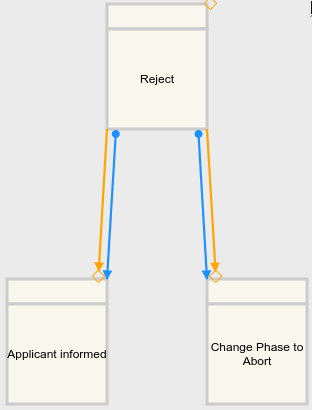
\includegraphics[width=0.8\linewidth]{images/dcrex1.png}
        \end{minipage}
    \end{frame}
    \begin{frame}[t]
        \frametitle{The Assignment}
        \framesubtitle{Part 1}
        We then model four patterns in the assignment.
    \end{frame}
    \begin{frame}[t]
        \frametitle{Pattern 1}
        \framesubtitle{Fill out Application}
        \begin{figure}[!h]
            \centering
            
\includegraphics[height=5cm]{images/dcpat1.png}
            \caption{Fill out application must come before the rest of the graph}
            \label{fig:a1}
        \end{figure}
    \end{frame}
    \begin{frame}[t]
        \frametitle{Pattern 2}
        \framesubtitle{Reject should always eventually be followed by "Applicant
        informed" and "Change phase to Abort"}
        \begin{figure}[!h]
            \centering
            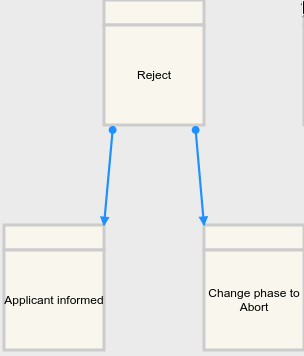
\includegraphics[height=5cm]{images/dcpat2.png}
            \caption{Using the Response relation}
            \label{fig:a2}
        \end{figure}
    \end{frame}
    \begin{frame}[t]
        \frametitle{Pattern 3}
        \framesubtitle{First Payment must only occur once}
        \begin{figure}[!h]
            \centering
            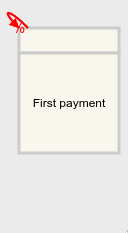
\includegraphics[height=5cm]{images/dcpat3.png}
            \caption{Excluding the sender}
            \label{fig:a3}
        \end{figure}
    \end{frame}
    \begin{frame}[t]
        \frametitle{Pattern 4}
        \framesubtitle{Only one of the reviews must occur at the same time}
        \begin{figure}[!h]
            \centering
            
\includegraphics[height=5cm]{images/dcpat4.png}
            \caption{Excluding another activity}
            \label{fig:a4}
        \end{figure}
    \end{frame}
    \begin{frame}[t]
        \frametitle{Conformance Checking}
        \framesubtitle{Additions To a handed-out DCR Implementation}
        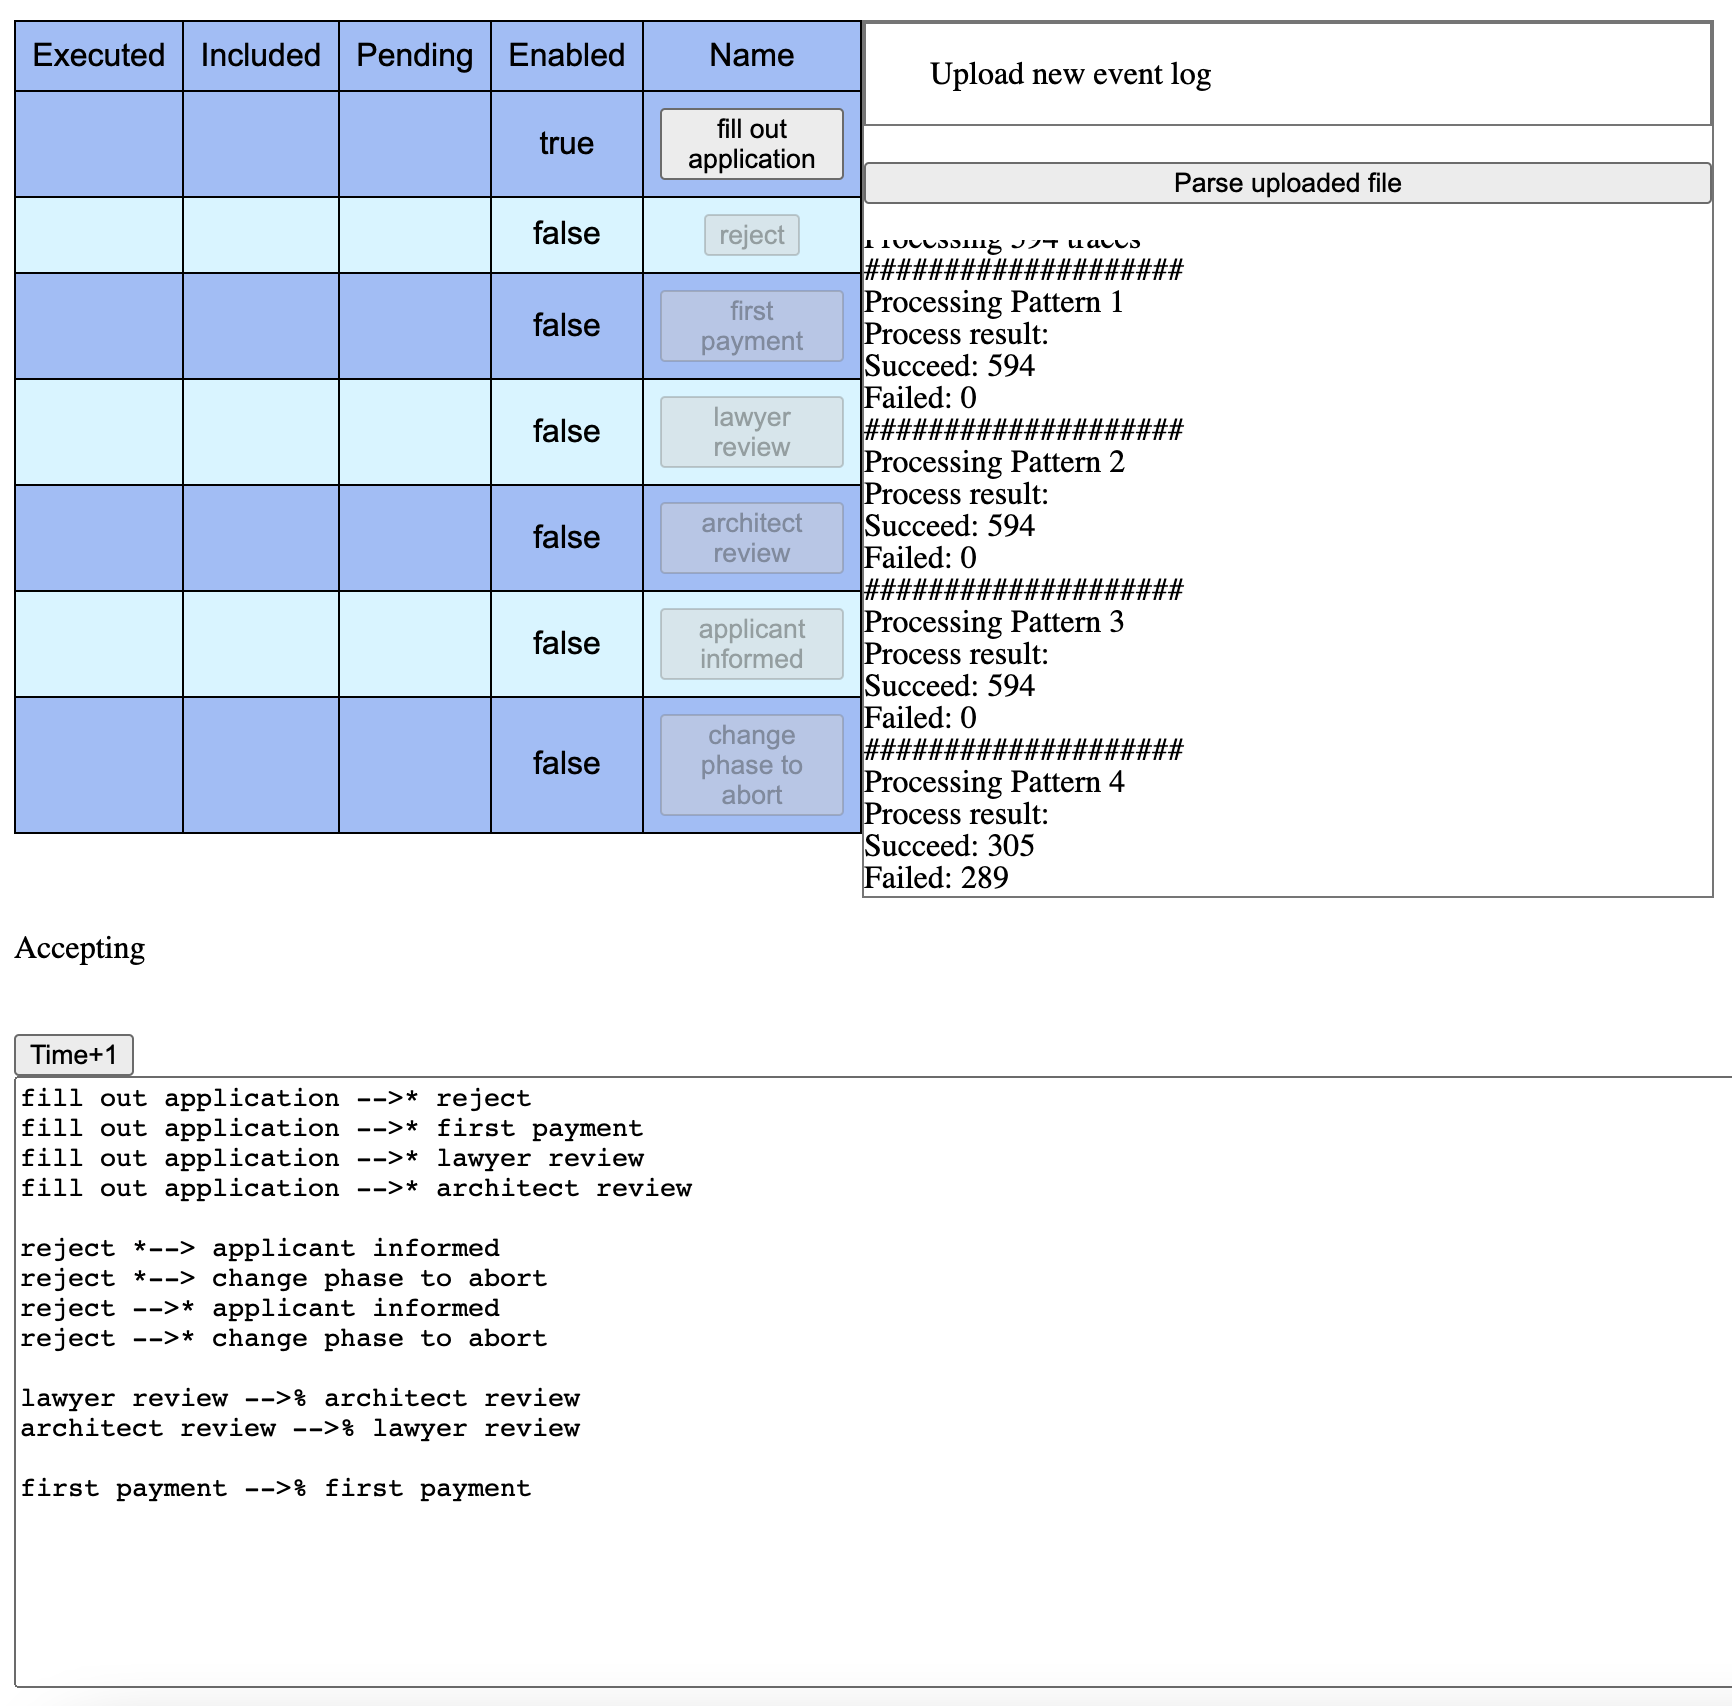
\includegraphics[width=\linewidth]{images/conformance.png}
    \end{frame}
    \begin{frame}[t]
        \frametitle{This Slide}
        \framesubtitle{Intentionally left blank}
    \end{frame}

    %_    ____  
   %/ \  |___ \ 
  %/ _ \   __) |
 %/ ___ \ / __/ 
%/_/   \_\_____|
    \section{Assignment 2}
    \begin{frame}[t]
        \frametitle{Part 2 of the Course - CCS Choreographies and Jolie}
        \framesubtitle{introduction}
        \begin{itemize}
            \item Changing focus a bit % From modelling business processing to reactive systems
            \item Choreographies and Jolie
        \end{itemize}
        
\includegraphics[width=0.2\linewidth]{images/jolielang.png}
    \end{frame}
    \begin{frame}[t]
        \frametitle{Modelling Buyers, Sellers, and Shippers}
        \framesubtitle{The interface Diagram}
        \begin{figure}
            \centering
            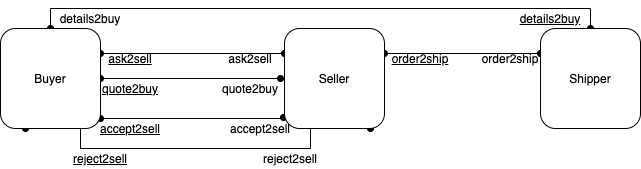
\includegraphics[width=0.8\linewidth]{images/InterfaceDiagram.png}
        \end{figure}
    \end{frame}
    \begin{frame}[t]
        \frametitle{Ports used}
        \framesubtitle{3 static and 1 dynamic port used}
        \begin{table}[!htb]
            \centering
            \begin{tabular}{l | r | r}
                Port & Input   & Output \\\hline
                8000 & Buyer   & Seller \\
                8001 & Buyer   & Shipper\\
                8002 & Shipper & Seller \\\hline
                9000+& Seller  & Buyer
            \end{tabular}
            \caption{The port table. The input column is which service defines the port as an inputport, 
            the output column describes who outputs to this port}
            \label{tab:portmap}
        \end{table}
        
    \end{frame}
    % Buyer
    \begin{frame}[t]
        \frametitle{Buyer}
        \framesubtitle{Input and outputs}
\begin{figure}[!h]
    \centering
    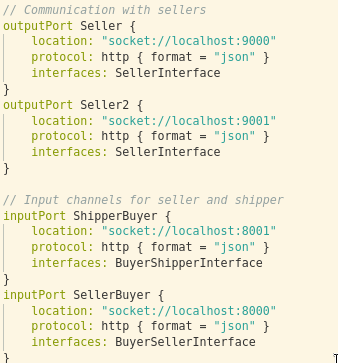
\includegraphics[height=5cm]{images2/buyerio.png}
    \caption{Outputs and Inputs, is this O/I}
    \label{fig:a2p1}
\end{figure}
    \end{frame}
    \begin{frame}[t]
        \frametitle{Buyer}
        \framesubtitle{Business Logic}
\begin{figure}[!h]
    \centering
    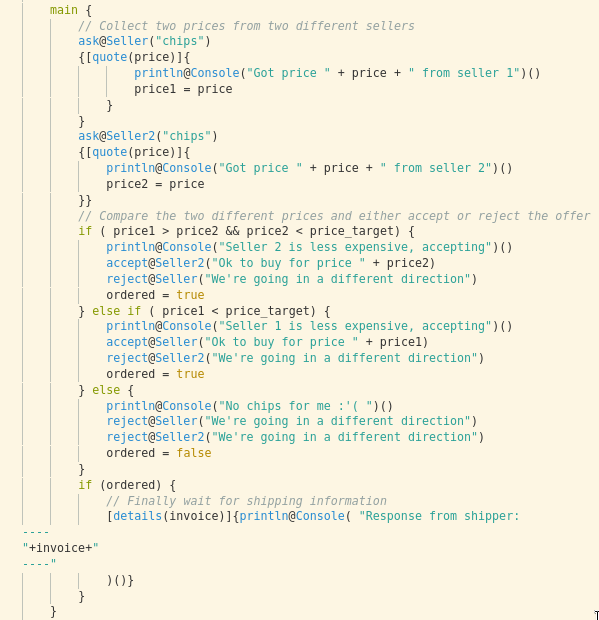
\includegraphics[height=5cm]{images2/buyerlogic.png}
    \caption{This isn't the smartest solution \emph{nor} the dumbest}
    \label{fig:a2p1}
\end{figure}
    \end{frame}

    % Seller
    \begin{frame}[t]
        \frametitle{Seller}
        \framesubtitle{Input and outputs}
\begin{figure}[!h]
    \centering
    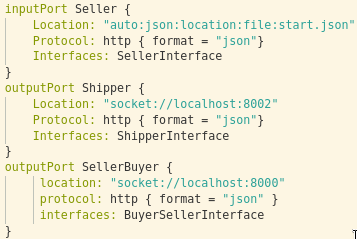
\includegraphics[height=5cm]{images2/sellerio.png}
    \caption{Notice the dynamic location}
    \label{fig:a2p2}
\end{figure}
    \end{frame}
    \begin{frame}[t]
        \frametitle{Seller}
        \framesubtitle{Business Logic}
\begin{figure}[!h]
    \centering
    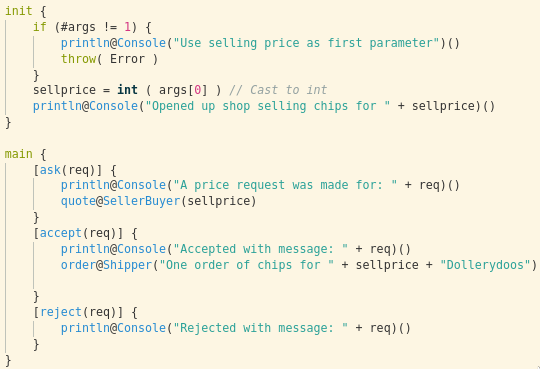
\includegraphics[height=5cm]{images2/sellerlogic.png}
    \caption{Main and init is quite simple to write despite the logic involved}
    \label{fig:a2p2}
\end{figure}
    \end{frame}

    % Shipper
    \begin{frame}[t]
        \frametitle{Shipper}
        \framesubtitle{Input and outputs}
\begin{figure}[!h]
    \centering
    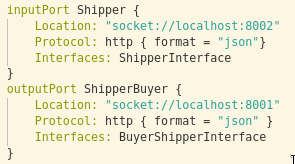
\includegraphics[height=5cm]{images2/shipperio.png}
    \caption{Doesn't need to know sellers location}
    \label{fig:a2p2}
\end{figure}
    \end{frame}
    \begin{frame}[t]
        \frametitle{Shipper}
        \framesubtitle{Business Logic}
\begin{figure}[!h]
    \centering
    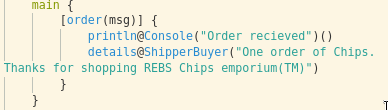
\includegraphics[width=8cm]{images2/shipperlogic.png}
    \caption{We don't actually ship anything }
    \label{fig:a2p2}
\end{figure}
    \end{frame}
    \begin{frame}[t]
        \frametitle{This Slide}
        \framesubtitle{Intentionally left blank}
    \end{frame}

    %_    _____ 
   %/ \  |___ / 
  %/ _ \   |_ \ 
 %/ ___ \ ___) |
%/_/   \_\____/ 
    \section{Assignment 3}
    \begin{frame}[t]
        \frametitle{Jolie, MQTT and how to tie them together}
        \framesubtitle{introduction}
        \begin{itemize}
            \item Message Queuing Telemetry Transport (MQTT)
            \item A subscriber-based communications protocol
        \end{itemize}
    \end{frame}
    \begin{frame}[t]
        \frametitle{A Filtered Subscriber}
        \framesubtitle{Input and outputs}
        \begin{figure}[!h]
            \centering
            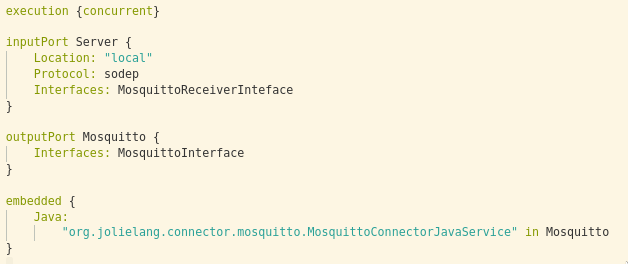
\includegraphics[height=5cm]{images3/filterio.png}
            \caption{Notice the mosquitto interfaces}
            \label{fig:a3p1}
        \end{figure}
    \end{frame}
    \begin{frame}[t]
        \frametitle{A Filtered Subscriber}
        \framesubtitle{Business Logic}
        \begin{figure}[!h]
            \centering
            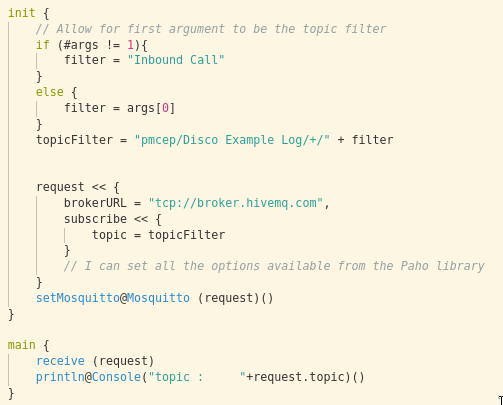
\includegraphics[height=5cm]{images3/filterlogic.png}
            \caption{Takes filters from the command line}
            \label{fig:a3p1}
        \end{figure}
    \end{frame}

    \begin{frame}[t]
        \frametitle{Making the whole thing a bit more interesting}
        \framesubtitle{Parsing the MQTT response}
        \textbf{What did we do:}   
        \begin{itemize}
            \item Subscribe to a specific topic
            \item Notify the stdout everytime an activity comes in
            \item Show off our different wildcards
        \end{itemize}
        \textbf{Whats next}   
        \begin{itemize}
            \item Responses are in json
            \item Jolie has global variables
            \item Jolie has File IO
        \end{itemize}
    \end{frame}
    \begin{frame}[t]
        \frametitle{A Counting Subscriber}
        \framesubtitle{Input and outputs}
        \begin{figure}[!h]
            \centering
            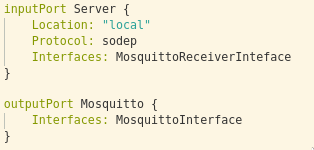
\includegraphics[height=5cm]{images3/countio.png}
            \caption{Same as previous subscriber}
            \label{fig:a3p2}
        \end{figure}
    \end{frame}
    \begin{frame}[t]
        \frametitle{A Counting Subscriber}
        \framesubtitle{Business Logic}
        \begin{figure}[!h]
            \centering
            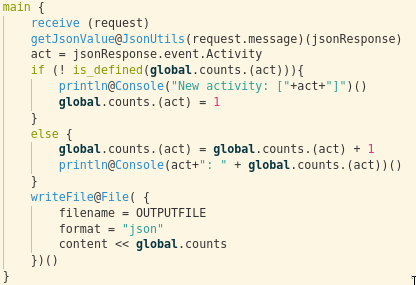
\includegraphics[height=5cm]{images3/countlogic.png}
            \caption{Our main function has tripled in size}
            \label{fig:a3p2}
        \end{figure}
    \end{frame}

    \begin{frame}[t]
        \frametitle{Plotting the results}
        \framesubtitle{People Call more than they email}
        \begin{figure}[!h]
            \centering
            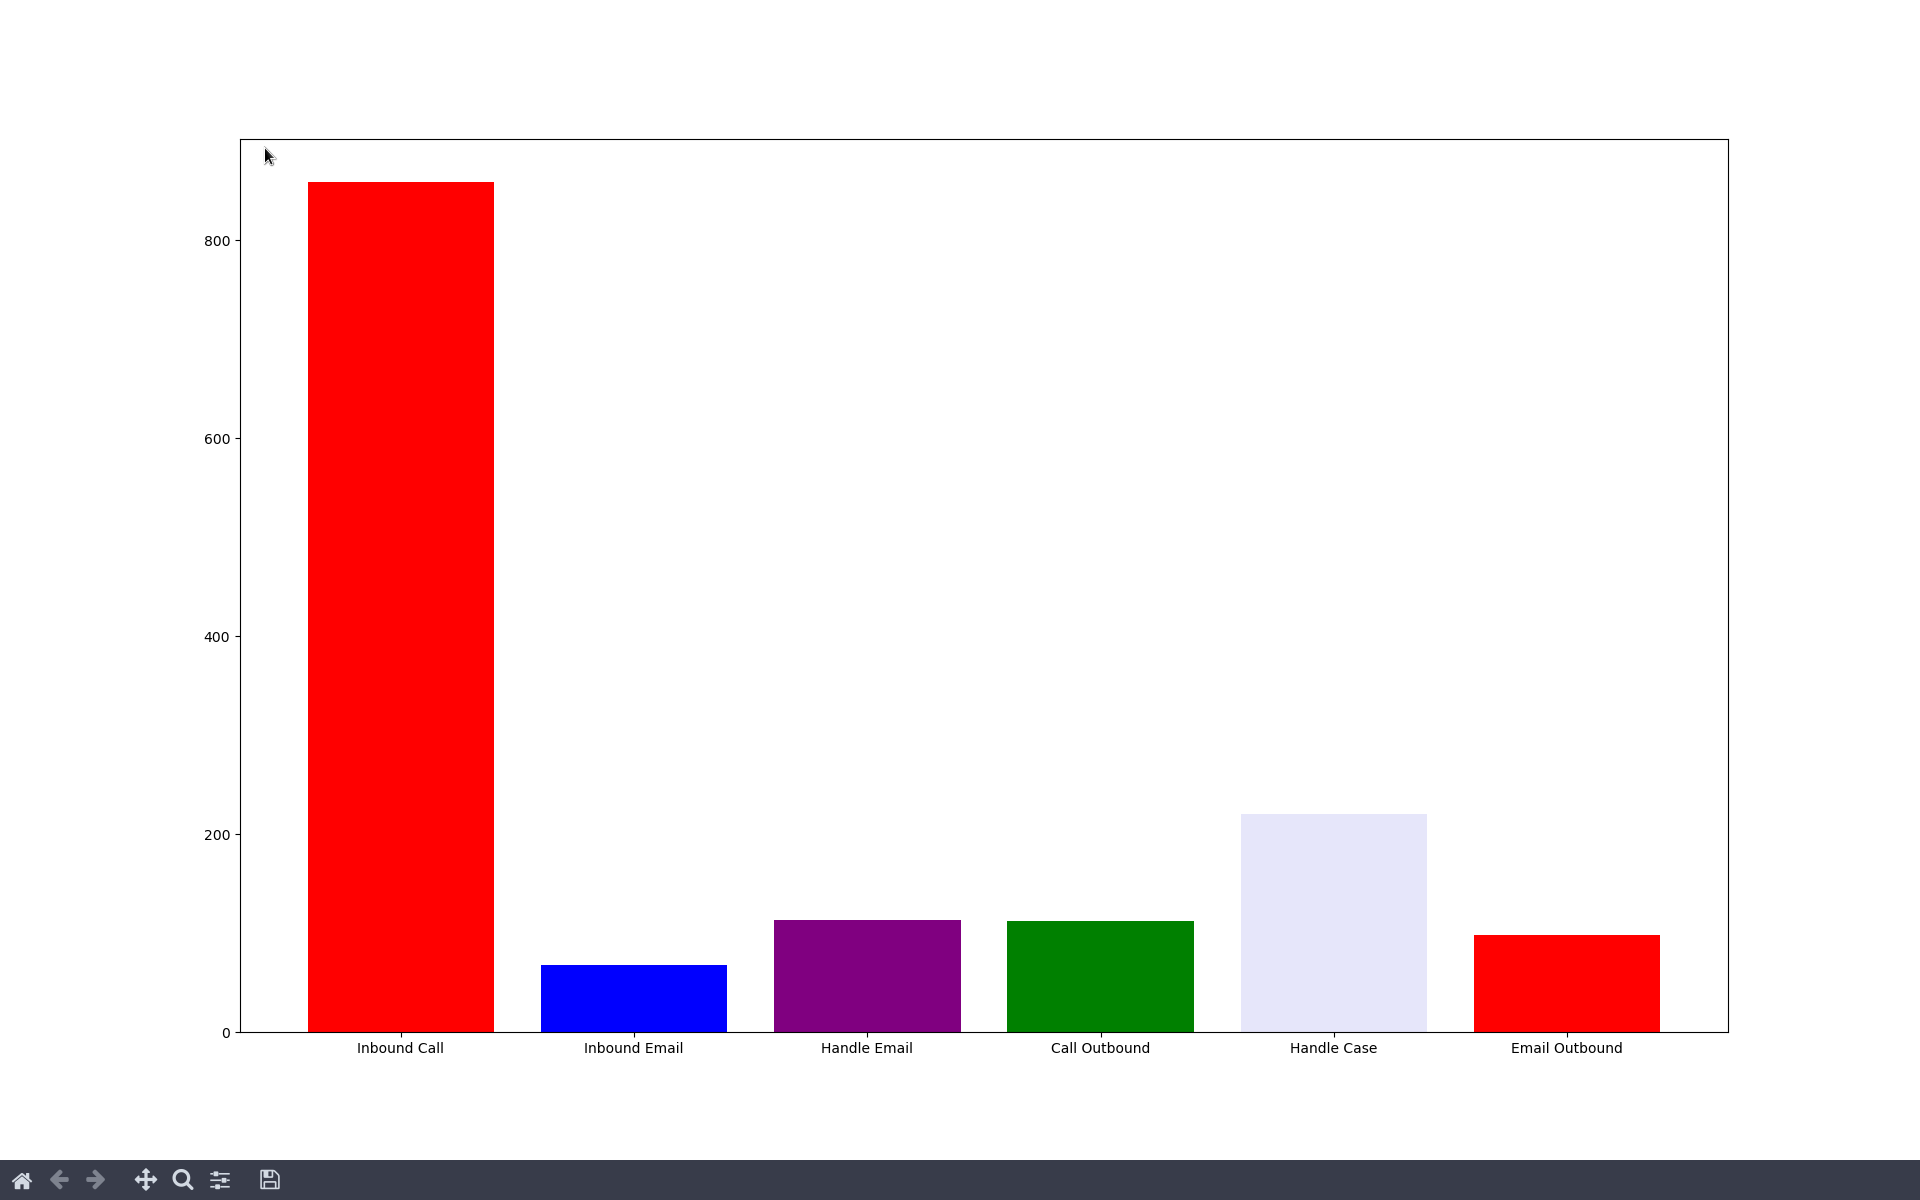
\includegraphics[width=1.0\linewidth]{images3/plot.png}
        \end{figure}
    \end{frame}

    \begin{frame}[t]
        \frametitle{This Slide}
        \framesubtitle{Intentionally left blank}
    \end{frame}


\end{document}
